\section{An\'alisis de resultados}\label{sec:analisis}
Una vez que el algoritmo est\'a totalmente desarrollado y es funcional, se lanzan un compendio de ejecuciones con distintas combinaciones de par\'ametros con el objetivo de ver cu\'an bueno es.
En un intento de mejorar la comprensi\'on de todas las ejecuciones realizadas, se va a dividir esta secci\'on en dos ep\'igrafes. \\

En el primero de ellos se hace un an\'alisis de los resultados obtenidos haciendo variaciones en los par\'ametros del algoritmo gen\'etico. Estos son el n\'umero de \'arboles, el n\'umero de iteraciones y el tipo de periodo.\\

M\'as tarde, en el segundo ep\'igrafe, se van a comparar los resultados obtenidos, a trav\'es de los mejores par\'ametros, con otro algortimo de naturaleza parecida desarrollado en Mousavi (2014).\\

De aqu\'i en adelante, se muestra varias tablas de resultados. Todas ellas muestran los beneficios obtenidos calculados con \textit{RoR}\footnote{RoR (Rate of Return) es una forma de calcular beneficios bastante com\'un en el mundo de la bolsa. As\'i pues, en lugar de mostrar los beneficios netos de la inversi\'on, se muestra el porcentaje de dinero perdido o ganado respecto al presupuesto inicial. Esto es, si se comienza con 10000 euros y se gana un 5\%, la ganacia neta es de 500 euros.}.

\subsection{An\'alisis de par\'ametros}

Para medir el rendimiento del algoritmo en distintas situaciones, se han propuestos varios periodos de diferente longitud y que presentan distintas tendencias. Por sencillez, todos han sido seleccionados del mismo valor de bolsa, \textit{Banco Santander}.\\

Para obtener una mejor comprensi\'on, se han definido cinco configuraciones de par\'ametros. Cada configuraci\'on tiene sus par\'ametros establecidos en la figura \ref{fig:params}. Estas configuraciones, dependiendo de la longitud del periodo, pueden tardar desde unos minutos en ejecutar hasta cuatro horas en el caso m\'as grande.\\

     	\begin{figure}[H]
     		\centering\leftskip=52px
     		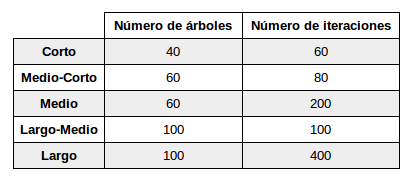
\includegraphics[scale=0.65]{imagenes/params.png}
     		\caption[Configuraciones de par\'ametros]{Configuraciones de par\'ametros.\\ Fuente: elaboraci\'on propia}
     		\label{fig:params}
     	\end{figure}

N\'otese que estas aproximaciones de tiempo ejecuci\'on se aportan a partir de la m\'aquina disponible, en este caso, de cuatro n\'ucleos y 3.4GHz.\\

En los casos expuestos a continuaci\'on se sigue siempre el mismo procedimiento. En primer lugar, el algoritmo gen\'etico efect\'ua, con los par\'ametros correspondientes, una serie de ejecuciones que terminan con una poblaci\'on evolucionada. De esta poblaci\'on obtenida, se selecciona el mejor de los individuos y se prueba tanto en el periodo de entrenamiento como en el periodo de prueba.\\

\subsubsection{Periodo largo}

En la primera de las ejecuciones, el periodo de entrenamiento comprende desde el 1 de abril de 2012 hasta el 1 de enero de 2016, por tanto, corresponde con un periodo bastante largo. De forma coherente, el periodo de prueba empieza el 1 de enero de 2016 y finaliza el 1 de mayo de 2019. Al comparar los perfiles de los precios en sendos periodos en las gr\'aficas, que se muestran a continuaci\'on, se puede observar que son parecidos, lo que deber\'ia mejorar los resultados.\\

     	\begin{figure}[H]
     		\centering\leftskip=-75px
     		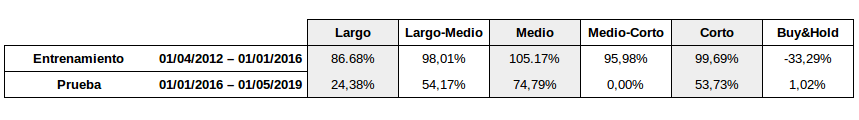
\includegraphics[scale=0.60]{imagenes/Large_period.png}
     		\caption[Ejecuci\'on en un periodo largo ascendente-descendente]{Ejecuci\'on en un periodo largo ascendente-descendente. Las cantidades mostradas son el porcentaje de beneficio respecto al presupuesto inicial.\\ Fuente: elaboraci\'on propia}
     		\label{fig:large_period}
     	\end{figure}
     	
A priori puede parecer que los resultados, que se pueden ver en la figura \ref{fig:large_period} son muy buenos. Pero, en realidad, muestran algunas carencias que se hacen realidad cuando se mira con detenimiento el calendario de inversi\'on.\\

Lo primero que destaca en la figura \ref{fig:large_period_mtrain}, que representa el calendario de inversi\'on del algoritmo con par\'ametros de perfil medio en el periodo de entrenamiento, es que la gran mayor\'ia de las ganancias proviene de una \'unica compraventa. El resto de inversiones son de poca duraci\'on y apenas si producen ganancias. La causa de este hecho puede ser una falta de especializaci\'on. Debido a la larga duraci\'on de la ejecuci\'on, cuatro a\~nos, es bastante complicado caracterizar por medio de indicadores los momentos buenos para comprar. Por tanto, es posible que, en lugar de buscar cada uno de los momentos de compra, el algoritmo solo sea capaz de encontrar instantes con caracter\'isticas muy dr\'asticas.\\

Es claro que, una inversi\'on de compra y venta algo m\'as r\'apida nos habr\'ia aportado una mayor ganacia.\\

Cuando analizamos el periodo de prueba, representado en la figura \ref{fig:large_period_mtest}, obtenemos un perfil similar. Se ha ajustado de manera muy eficiente una \'unica compraventa. Si bien es cierto que esa transacci\'on es casi perfecta, hay otras transacciones v\'alidas que no se han ejecutado.\\

     	\begin{figure}[H]
     		\centering\leftskip=30px
     		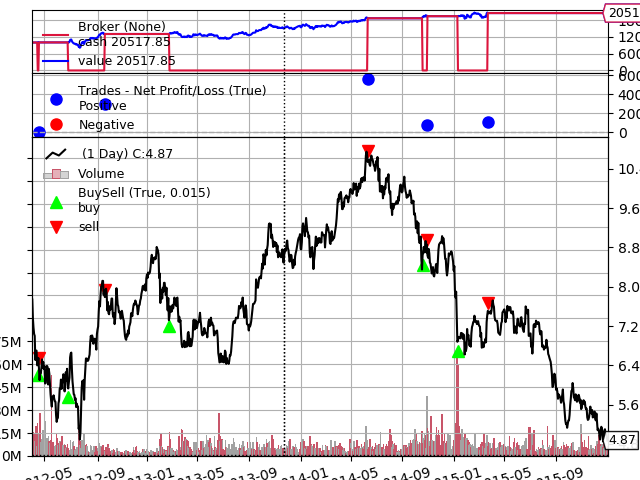
\includegraphics[scale=0.70]{imagenes/L_Medium_train.png}
     		\caption[Calendario de inversi\'on del periodo de entrenamiento largo.]{Calendario de inversi\'on del periodo de entrenamiento largo con par\'ametros de perfil Medio.\\ Fuente: elaboraci\'on propia}
     		\label{fig:large_period_mtrain}
     	\end{figure}
     	
     	\begin{figure}[H]
     		\centering\leftskip=30px
     		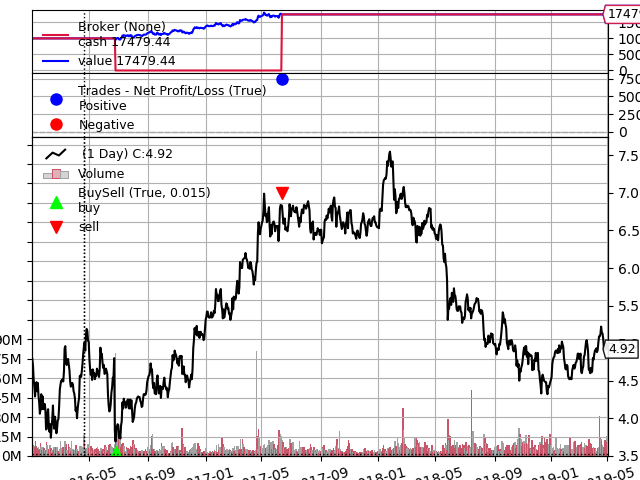
\includegraphics[scale=0.70]{imagenes/L_Medium_test.png}
     		\caption[Calendario de inversi\'on del periodo de prueba largo]{Calendario de inversi\'on del periodo de prueba largo con par\'ametros de perfil Medio.\\ Fuente: elaboraci\'on propia}
     		\label{fig:large_period_mtest}
     	\end{figure}     	

En resumen, los peridos largos dan muchas posibilidades de compraventa que nuestro algoritmo no puede aprovechar. La parte positiva es que la mayor\'ia de las veces, cuando invierte, lo hace con beneficio. No obstante, en ocasiones, puede que no invierta y tengamos un modelo f\'util, como es el caso de la ejecuci\'on de par\'ametros de perfil Medio-Corto. Las simulaciones con periodos largos no parecen demasiado beneficiosas.\\

\subsubsection{Periodo medio}

En este segundo caso, se han elegido dos periodos distintos. En el primer periodo, claramente alcista, el entrenamiento comprende desde el 29 de septiembre de 2002 hasta el 29 de septiembre de 2003. Por otro lado, el periodo de prueba empieza el 29 de septiembre de 2003 y finaliza el mismo d\'ia de 2004. \\

El segundo periodo, de car\'acter bajista, est\'a formulado tambi\'en de a\~no en a\~no, el entrenamiento comienza el 1 de noviembre de 2009 y la prueba empieza el 1 de noviembre de 2010.\\

Una vez m\'as, se han tomado fechas en las que los perfiles de los precios se asemejan pero, en esta simulaci\'on, no son iguales. \\

     	\begin{figure}[H]
     		\centering\leftskip=-75px
     		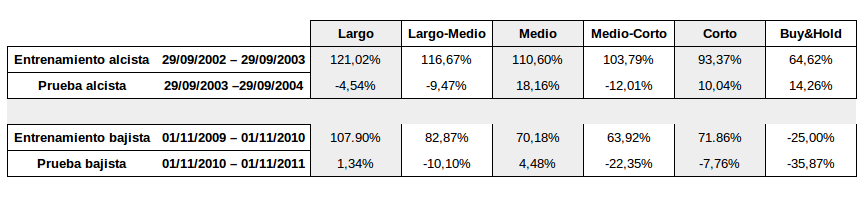
\includegraphics[scale=0.60]{imagenes/Medium_period.png}
     		\caption[Ejecuciones en un periodo medio alcista y en un periodo medio bajista]{Ejecuciones en un periodo medio alcista y en un periodo medio bajista. Las cantidades mostradas son el porcentaje de beneficio respecto al presupuesto inicial.\\ Fuente: elaboraci\'on propia}
     		\label{fig:medium_period}
     	\end{figure}
     	
En esta ocasi\'on, los resultados son algo peores. Con motivo de ilustrar la adaptaci\'on de los modelos obtenidos en el periodo de entrenamiento, se han tomado periodos de prueba ligeramente peores, es decir, el precio tiende, significativamente, a bajar m\'as que en el entrenamiento.\\

En todos los casos, el modelo obtenido con el algoritmo gen\'etico fue mejor que la estrategia \textit{Buy\&Hold} evaluados en el periodo de entrenamiento. Esto quiere decir que el algoritmo es capaz de encontrar condiciones de compra y venta que reportan beneficios en el periodo de aprendizaje. Sin embargo, estas condiciones no devuelven buenos resultados en periodos ligeramente distintos. De hecho, incluso en periodos alcistas, se pierde dinero cuando el modelo en el entrenamiento consigue sacar un 121.02\% de beneficios.\\

Otro punto que se puede destacar es la irregularidad del algoritmo. Habitualmente, otros algoritmos tienden a sobreaprender cuando se insiste demasiado en los datos de entrenamiento. As\'i pues, es habitual encontrar un punto de entrenamiento a partir del cual los resultados obtenidos en las pruebas empeoran.\\

En este algoritmo propuesto, los resultados obtenidos  para el periodo de prueba parecen variar de forma independiente al periodo anterior. Tras m\'ultiples ejecuciones con los mismos par\'ametros se puede observar como, en ocasiones, los resultados var\'ian de forma significativa. Este hecho puede ser la causa de la aleatoriedad en el algoritmo debida a, posiblemente, la gran cantidad de mutaciones necesarias y la aleatoriedad de la primera generaci\'on.\\

     	\begin{figure}[H]
     		\centering\leftskip=40px
     		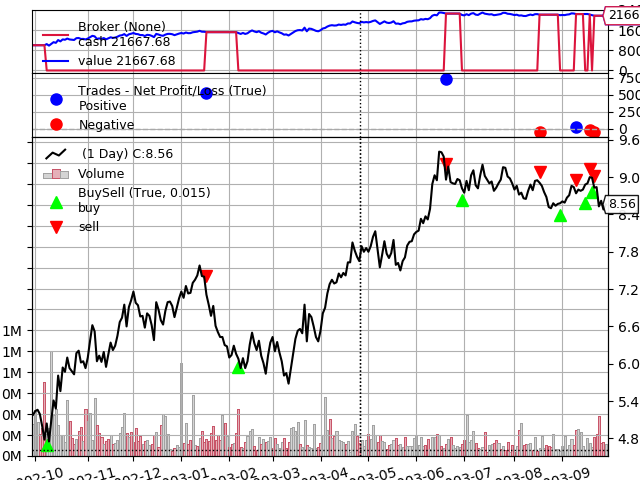
\includegraphics[scale=0.66]{imagenes/M_Large-Medium_train.png}
     		\caption[Calendario de inversi\'on del periodo de entrenamiento largo.]{Calendario de inversi\'on del periodo de entrenamiento alcista, longitud media y con par\'ametros de perfil Largo-Medio.\\ Fuente: elaboraci\'on propia}
     		\label{fig:medium_period_mtrain}
     	\end{figure}
     	
     	\begin{figure}[H]
     		\centering\leftskip=40px
     		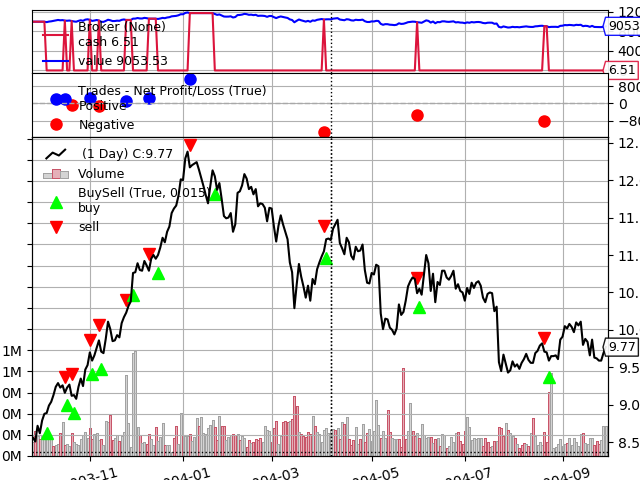
\includegraphics[scale=0.66]{imagenes/M_Large-Medium_test.png}
     		\caption[Calendario de inversi\'on del periodo de prueba medio]{Calendario de inversi\'on del periodo de prueba alcista, longitud media y con par\'ametros de perfil Largo-Medio.\\ Fuente: elaboraci\'on propia}
     		\label{fig:medium_period_mtest}
     	\end{figure} 

Por otro lado, en las figuras \ref{fig:medium_period_mtrain} y \ref{fig:medium_period_mtest}, puede observarse bastante bien esta la adaptaci\'on. En el periodo de entrenamiento se hacen varias inversiones de unas semanas, e incluso de varios meses, entre las cuales se deja un margen de tiempo hasta que es un buen momento de compra. Por el contrario, en el periodo de prueba apenas si hay unas semanas en las que el modelo no tiene nada comprado, es decir, siempre que vende intenta comprar inmediatamente.\\

Se considera, como consecuencia de este hecho, la hip\'otesis de que el algoritmo tiene un buen aprendizaje pero una mala adaptaci\'on a otros periodos.\\

     	
\subsubsection{Periodo corto}

Para la \'ultima de las ejecuciones de par\'ametros, se han escogido tambi\'en dos periodos pero, esta vez, se ha tomado un periodo alcista y un periodo lateral. Este segundo es algo complicado, pues el periodo de entrenamiento es lateral pero el de prueba tiene tendencia bajista. \\

En primer lugar, el periodo alcista tiene su entrenamiento desde el 1 de julio de 2016 y hasta el 22 de octubre de 2016. Por otro lado, el periodo de prueba empieza a partir de entonces y hasta el 1 de febrero de 2017.\\

En segundo lugar, el periodo lateral comprende un poco m\'as de tres meses. El periodo de entrenamiento empieza el 1 de enero de 2018 y, por su parte, el periodo de prueba comienza el 22 de abril de 2018. La simulaci\'on termina, finalmente, el 22 de julio de 2018. Como ya se ha adelantado, no se esperan buenos resultados. Los modelos generados tienen poca capacidad de adaptaci\'on y, como hemos tomado periodos de entrenamiento y prueba con perfiles muy distintos, la adaptaci\'on debe ser peor.\\

     	\begin{figure}[H]
     		\centering\leftskip=-75px
     		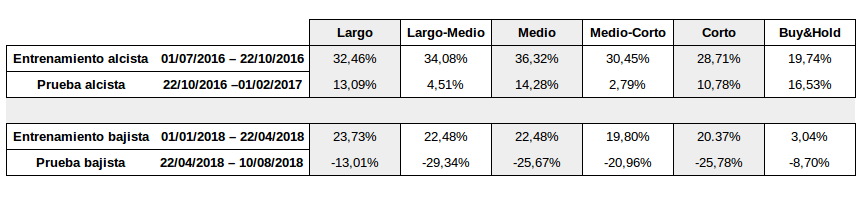
\includegraphics[scale=0.60]{imagenes/Short_period.png}
     		\caption[Ejecuciones en un periodo corto alcista y en un periodo corto lateral]{Ejecuciones en un periodo corto alcista y en un periodo corto lateral. Las cantidades mostradas son el porcentaje de beneficio respecto al presupuesto inicial.\\ Fuente: elaboraci\'on propia}
     		\label{fig:short_period}
     	\end{figure}

Como se observa en la figura \ref{fig:short_period}, en los periodos cortos no se obtienen buenos resultados. De hecho, en el caso del periodo lateral, y prueba bajista, los resultados son negativos. Mientras que, en el entrenamiento, la estrategia propia supera con creces a la estrategia \textit{Buy\&Hold}, en la prueba tiene p\'erdidas estrepitosas al ser un periodo bajista. Esto confirma la hip\'otesis de la baja adaptaci\'on del algoritmo.\\

     	\begin{figure}[H]
     		\centering\leftskip=30px
     		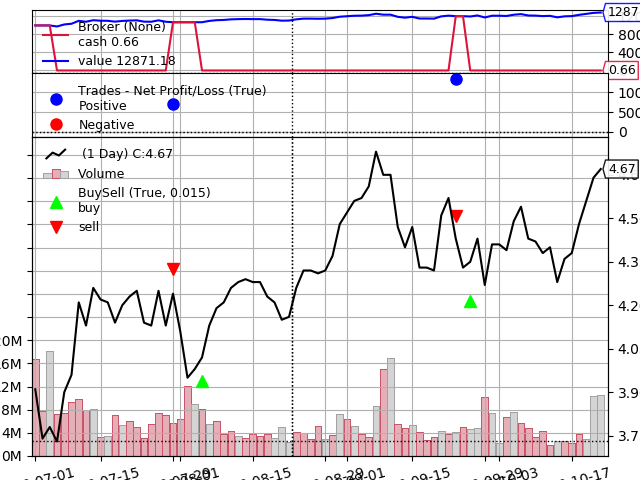
\includegraphics[scale=0.70]{imagenes/S_Short_train.png}
     		\caption[Calendario de inversi\'on del periodo de entrenamiento corto alcista.]{Calendario de inversi\'on del periodo de entrenamiento corto y alcista con perfil de par\'ametros Corto.\\ Fuente: elaboraci\'on propia}
     		\label{fig:short_period_uptrain}
     	\end{figure}
     	
En la figura \ref{fig:short_period_uptrain}, correspondiente al periodo alcista de entrenamiento, se encuentra un modelo generado con perfil de par\'ametros corto que invierte de una forma muy eficiente, esto es, compra en los m\'inimos y vende en los m\'aximos. \\

Teniendo esta regla como referencia, se analiza el mismo modelo ejecutado, esta vez, en el periodo de prueba en la figura \ref{fig:short_period_uptest}. Este periodo tiene un perfil de precio distinto, los m\'inimos y m\'aximos no son tan destacables. No obstante, el algoritmo ha generado un modelo que, tal y como se intuye, est\'a intentando hacer algo similar a lo realizado en el periodo del que aprendi\'o. Las primeras transacciones son torpes y demasiado abundantes, produciendo p\'erdidas con las comisiones.	Por tanto, a pesar de ser un periodo alcista, no tiene tanto \'exito como la estrategia de \textit{Buy\&Hold}.\\
     	
     	\begin{figure}[H]
     		\centering\leftskip=30px
     		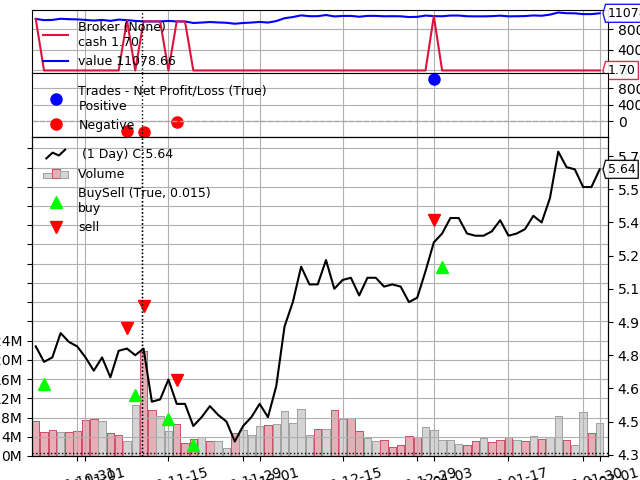
\includegraphics[scale=0.70]{imagenes/S_Short_test.png}
     		\caption[Calendario de inversi\'on del periodo de prueba corto alcista]{Calendario de inversi\'on del periodo de prueba corto y alcista con perfil de par\'ametros Corto.\\ Fuente: elaboraci\'on propia.}
     		\label{fig:short_period_uptest}
     	\end{figure} 
     	
Por \'ultimo, se propone hacer una an\'alisis del periodo entrenado con perfil lateral pero probado con un perfil bajista. Las figuras \ref{fig:short_period_downtrain} y \ref{fig:short_period_downtest} contiene los calendarios de inversi\'on de estas simulaciones realizadas con configuraci\'on de par\'ametros Largo.\\

En el entrenamiento se tiene una inversi\'on muy ajustada, pr\'acticamente inmejorable. No obstante, esto podr\'ia ser fruto de un sobreaprendizaje. Por su parte, en el periodo de prueba, se observan los mismos patrones de compra y venta. Pero al ser las oscilaciones del precio m\'as peque\~nas que en el caso anterior, las comisiones se llevan esos escasos beneficios que pudiera tener.\\

En contraposici\'on, encontramos un punto a favor, la precisi\'on para encontrar los m\'inimos. Los indicadores parecen ser unas buenas herramientas para detectar estos. N\'otese que, tras una acentuada ca\'ida durante el primer mes, se compra en el \'ultimo momento antes de la subida. Por tanto, aunque los resultados no sean correctos, las se\~nales de compra y venta no son demasiado err\'oneas. \\
     	
      	\begin{figure}[H]
      		\centering\leftskip=40px
      		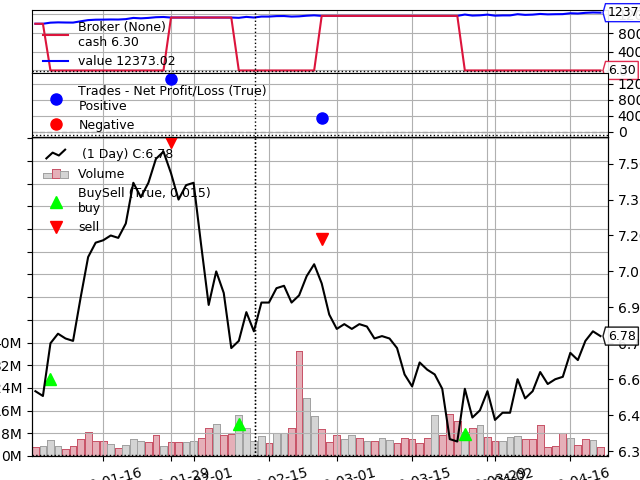
\includegraphics[scale=0.66]{imagenes/S_Large_train.png}
      		\caption[Calendario de inversi\'on del periodo de entrenamiento corto lateral]{Calendario de inversi\'on del periodo de entrenamiento corto lateral con perfil de par\'ametros Largo.\\ Fuente: elaboraci\'on propia.}
      		\label{fig:short_period_downtrain}
      	\end{figure}
      	
     	\begin{figure}[H]
     		\centering\leftskip=40px
     		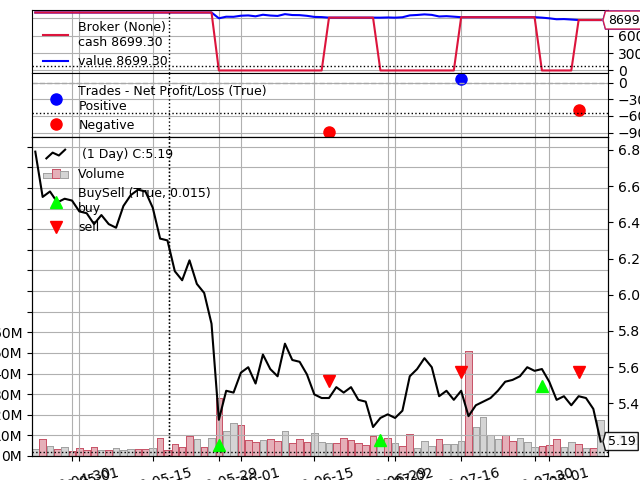
\includegraphics[scale=0.66]{imagenes/S_Large_test.png}
     		\caption[Calendario de inversi\'on del periodo de prueba corto bajista]{Calendario de inversi\'on del periodo de prueba corto bajista con perfil de par\'ametros Largo.\\ Fuente: elaboraci\'on propia.}
     		\label{fig:short_period_downtest}
     	\end{figure} 

\subsection{Contraste con otra estrategia}

Con el objetivo de comparar el algoritmo desarrollado con otras estrategias, se ha propuesto realizar el siguiente experimiento. Se han tomado 13 empresas que cotizan en la bolsa de Toronto (Canad\'a). Y se han marcado cuatro periodos, de seis meses cada uno, para simular la inversi\'on en bolsa. Para invertir en cada etapa se ha entrenado con el periodo de seis meses inmediatamente anterior.\\

A continuaci\'on, se muestra la comparativa de los beneficios de nuestro algoritmo con los obtenidos por la estrategia cl\'asica \textit{Buy\&Hold} y el modelo gen\'etico de Mousavi (2014). La elecci\'on de estas dos estrategias no es casual. La primera de ellas es una estrateg\'ia b\'asica y, a partir de ella, es f\'acil ver si estamos simulando un periodo a la baja o al alza. La elecci\'on de la segunda estrategia tiene que ver con la similitud que guarda con la desarrollada. Aunque, en el algoritmo del art\'iculo un individuo son $n$ \'arboles juntos (uno por empresa a invertir), los cruces entre individuos se realizan de \'arbol i-\'esimo en \'arbol i-\'esimo, es decir, los \'arboles generados para distintas  empresa no se relacionan. Por tanto, los cruces son similares al modelo propuesto aqu\'i.\\

La diferencia principal con nuestro modelo radica en la construcci\'on de los \'arboles. A diferencia de nuestro caso, en el que los \'arboles son de decisi\'on, los \'arboles en el algoritmo de Mousavi representan funciones. Esto es, en los nodos se sit\'uan operaciones matem\'aticas y en las hojas, valores constantes o indicadores. Por consiguiente, se tiene la posibilidad de realizar operaciones con varios indicadores, pero encadenar m\'ultiples condiciones es m\'as inusual.

     	\begin{figure}[H]
     		\centering\leftskip=0px
     		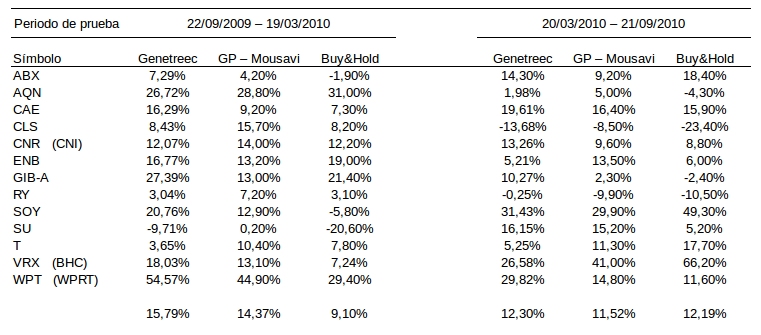
\includegraphics[scale=2]{imagenes/Mousavi1.png}
     		\caption[Comparaci\'on de resultados con Mousavi]{Comparaci\'on de resultados con Mousavi. Periodos 1 y 2. Algunas empresas han cambiado de nombre. Para localizarlas f\'acilmente se ha escrito su nombre actual entre par\'entesis. El algoritmo \textit{Genetreec} es el algoritmo propuesto en este proyecto.\\ Fuente: elaboraci\'on propia.}
     		\label{fig:Mousavi1}
     	\end{figure} 
     

En la figura \ref{fig:Mousavi1} se encuentran los resultados de los dos primeros periodos. En sendas ejecuciones se observa, con ayuda de los resultados obtenidos por \textit{Buy\&Hold}, que estamos en periodos crecientes. Adem\'as, los periodos de entrenamiento tambi\'en lo son. Estamos, pues, en la mejor situaci\'on posible para nuestro algoritmo. Los beneficios, en media, son mejores que los de las otras dos estrategias. Sin embargo, en los valores \textit{CLS} y \textit{RY} las ganacias son negativas en el segundo periodo y, en comparaci\'on con los beneficios de Mousavi, no son buenas cifras. En ambos casos se intuye el mismo problema, el periodo de entrenamiento es muy distinto al de prueba.\\

Como se adelantaba, las empresas que est\'an en periodos alcistas en los dos tramos son las que mejores beneficios reportan. Es el caso de \textit{WPT}, que en el primer caso obtiene un beneficio de 54,57\%.\\

Por otro lado, en los periodos 3 y 4, no se obtienen unos resultados tan buenos. El motivo, una vez m\'as, parece ser el gran cambio de tendencia. Por poner algunos ejemplo, en el tercer periodo \textit{CLS} pasa de perder un 23,4\% a ganar un 22\%, \textit{ABX} pasa de ganar un 18\% a perder algo m\'as de un 2\% y \textit{WPT} pasa de 11,6\% a -5,1\%.\\

En el caso del cuarto periodo, los cambios son a\'un m\'as notables. Se tienen como norma general unos resultados mejorables, a excepci\'on de \textit{WPT} que, de forma inesperada, gana un 34,39\% en unas condiciones desfavorables. De este resultado, en principio poco acorde con el resto, podemos extraer un nuevo detalle. Si el periodo de entrenamiento es bajista, pero el de prueba es alcista, el cambio de perfil no produce malos resultados. No obstante, si es al rev\'es, las p\'erdidas si que se producen.

     	\begin{figure}[H]
     		\centering\leftskip=0px
     		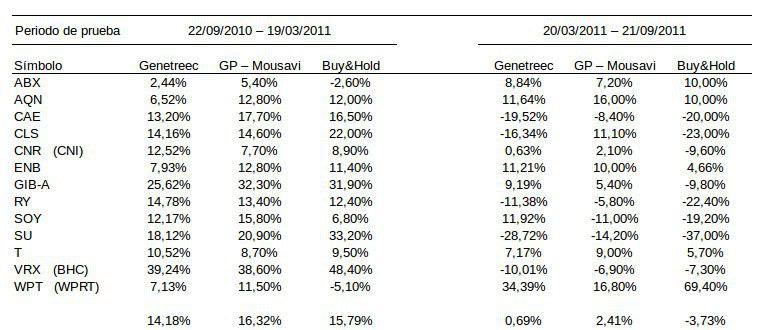
\includegraphics[scale=2]{imagenes/Mousavi2.jpg}
     		\caption[Comparaci\'on de resultados con Mousavi]{Comparaci\'on de resultados con Mousavi. Periodos 3 y 4. \\ Fuente: elaboraci\'on propia.}
     		\label{fig:Mousavi2}
     	\end{figure} 

\newpage
\section{Conclusiones}
Para finalizar este proyecto, se va a hacer una s\'intesis en la que repasaremos los objetivos que propusimos al inicio.\\

En primer lugar, se prentend\'ia realizar un estudio para utilizar t\'ecnicas de aprendizaje con algoritmos evolutivos basados en \'arboles para extraer informaci\'on de se\~nales de compra y venta. El dise\~no de este algoritmo se especifica en el punto \ref{sec:algorithm}. El c\'odigo que corresponde al dise\~no no se puede incluir en la memoria por motivos de espacio, no obstante, se incluye como anexo.\\

Adem\'as, debido al alto coste computacional de los modelos generados, se han realizado mejoras, detalladas en la secci\'on \ref{sec:timeimprove}, del software que mostraron una reducci\'on de tiempo considerable. En el caso de la ejecuci\'on m\'as larga, entrenamiento de cuatro a\~nos y prueba de tres con poblaci\'on de 100 \'arboles y 400 iteraciones, el tiempo total fue de algo menos de cuatro horas. La ejecuci\'on m\'as corta, por su parte, de tres meses de entrenamiento y otros tres de prueba con 40 \'arboles y 60 iteraciones, tuvo un tiempo de apenas dos minutos. Recordando que las ejecuciones fueron realizadas en un ordenador convencional de cuatro n\'ucleos y 3.4GHz, la eficiencia es satisfactoria.\\

En el segundo punto se marc\'o como objetivo analizar los resultados obtenidos en diferentes situaciones y, asimismo, comparar estos con otros resultados de la bibliograf\'ia. Gracias al desarrollo de la secci\'on \ref{sec:analisis} podemos considerar este objetivo cumplido. Al comparar los resultados con los obtenidos por Mousavi (2014), se encuentra un punto a favor. Este es que, en los periodos claramente alcistas o laterales con posibilidad de obtener ganacia, los beneficios son ligeramente mayores. No obstante, en las simulaciones en las que los periodos de entrenamiento son alcista y los de prueba son bajistas, el algoritmo no produce modelos tan eficientes como el propuesto en el art\'iculo. Consideramos, pues, condicionar la bondad del modelo a los periodos de simulaci\'on.\\



\subsection{Perfil del algoritmo}

A partir de las ejecuciones de la secci\'on \ref{sec:analisis}, se pueden distinguir varios casos en los que el algoritmo obtiene buenos resultados. Por otro lado, tambi\'en se distinguen casos en los que los resultados no son deseables.\\

Por lo general, los modelos aprenden muy bien de los periodos de entrenamiento. Esto produce una buena inversi\'on en el periodo de prueba siempre que las fluctuaciones de los precios sean similares en sendos periodos, especialmente si son alcistas o laterales. En las etapas claramente bajistas, el modelo aprendido suele producir condiciones que nunca llevan a comprar acciones, por lo que entrenar con este tipo de periodos no es aconsejable.\\

Si, en el caso contrario, los datos de entrenamiento y el periodo de inversi\'on tiene movimientos de precio muy dispares, el algoritmo suele producir algunas p\'erdidas.\\

Por tanto, el algoritmo es bastante eficaz en el caso de que nos aseguremos de que el periodo en el que se invierte es similar al periodo del que se aprende. Esta condici\'on, a priori deseable en todos los problemas de aprendizaje a partir de datos, es un problema com\'un en el mundo de la bolsa.

Por \'ultimo, hay que notar la aleatoriedad del modelo. La construcci\'on de los primeros \'arboles, el cruce de estos y las mutaciones producidas incorporan al modelo una gran cantidad de aleatoriedad. Esto produce que espacio de b\'usqueda sea inspeccionado de forma m\'as eficaz pero, a la hora de extraer un modelo, va a producir resultados distintos.

\subsection{Trabajos futuros}

Uno de los factores que se debe auxiliar en primer lugar es la baja adaptabilidad. Esta produce muchas p\'erdidas y es una caracter\'istica poco deseable para cualquier estrategia de bolsa. Para corregir este hecho se podr\'ia hacer un entrenamiento m\'ultiple, es decir, entrenar con varios periodos de distintos perfiles. De esta forma, las puntuaciones obtenidas por los \'arboles estar\'ian contrastadas en varios periodos, produciendo as\'i un mejor funcionamiento del modelo en el caso de cambio de tendencias.\\

Otra posibilidad para corregir estos sucesos podr\'ia ser auxiliar al modelo con otros algoritmos capaces de detectar los cambios de tendencia. De hecho, en el cl\'asico an\'alisis de indicadores, es com\'un utilizar algunos indicadores, como el \textit{RSI}, para percibir cambios de tendencia en los precios de las acciones. De esta forma, se podr\'ia crear una estrategia condicionada a las tendencias predichas. Si se espera una tendencia fija durante algunos meses, se usa el algoritmo desarrollado en el proyecto. En caso contrario, se puede usar un algoritmo especializado en los periodos irregulares. \\

Otra de las mejoras que se sugiere es realizar un modelo con varios \'arboles, imitando al algoritmo \textit{Random Forest}. Es posible que las se\~nales enviadas por la mayor\'ia de los individuos generados sean m\'as acertadas. Esto conlleva un problema, dado que existen tres etiquetas y las condiciones en los nodos pueden ser demasiado estrictas, los \'arboles podr\'ian no coincidir en muchos casos. Es m\'as, en muchos instantes primar\'ia la etiqueta \textit{Stop}, lo que produce estrategias f\'utiles.